%!TEX root = ../planets-notes.tex

\section{Declination and right ascension}
To talk about events in the sky, we need to specify where they are located. To specify where they are located, we need a point of reference.  This is a bit tricky: we are riding on the Earth, which rotates and orbits the Sun; the Sun orbits the Milky Way; the Milky Way moves through the Local Group; and on top of all this the universe is expanding.

The primary criterion for choosing a coordinate system is convenience. We want a system that is easy to use and that describes the sky straightforwardly.
As viewed from Earth, we appear to be at the center of a great sphere, with celestial objects lying on its surface. This is similar to describing locations on the Earth, for which we use two angles: latitude, which measures the angle north or south from the equator; and longitude, which measures the angle east or west from the prime meridian.  Likewise, to describe the apparent position of objects as viewed from Earth, we also need two angles.

\begin{marginfigure}
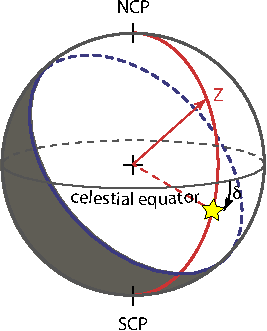
\includegraphics[width=\linewidth]{celestial-sphere}
\caption[The celestial sphere]{The meridian (red) passing through our zenith (Z).  Our vantage point is from the center of the sphere. Also shown are the north celestial pole (NCP), south celestial pole (SCP) and the celestial equator (CE).  The shaded region are points below our horizon; objects in that region are not visible from our location. A star with negative declination $\delta$ is shown as well.}
\label{f.meridian}
\end{marginfigure}

First, let's describe our measurement of position on the sky.
The local gravitational acceleration $\bvec{g}$ specifies the \emph{local vertical}; this picks out a point on the celestial sphere, our \emph{zenith}.  Our \emph{horizon} is then defined by points that lie $90^{\circ}$ from this zenith, measured along a great circle passing through the zenith.  The zeniths above the north and south poles define the \emph{north and south celestial poles}.  A great circle connecting the celestial poles and our zenith defines our \emph{meridian} (see Fig.~\ref{f.meridian}).  As the Earth rotates, celestial objects appear to move westward on circles about the celestial poles.  

Midway between the north and south celestial poles lies the celestial equator.  For any star, you specify its declination $\delta$ as the angle north (positive) or south (negative) of the celestial equator along that star's meridian.  For example, Betelgeuse, the red star in the shoulder of Orion, has a declination $\delta = \dec{7}{24}{25}$.  Polaris, the North star, has $\delta = \dec{89}{15}{51}$.
\marginnote{Declination is quoted in degrees ($^{\circ}$), arcminutes ($'$), and arcseconds ($''$).  There are 60 arcminutes in 1 degree and 60 arcseconds in 1 arcminute.}

\begin{exercisebox}[Altitude of Betelgeuse]
How far above our southern horizon will Betelgeuse be when it crosses our meridian? Our latitude is \dec{42}{43}{25}N.
\end{exercisebox}

Declination measures how far north or south of the celestial equator a given object lies. To specify an east-west location, we need another reference point.  Because of the Earth's rotation, we can't use a point on Earth, such as the Greenwich observatory (which is where the $0^{\circ}$ of longitude is defined).  We can, however, use the Earth's motion around the Sun: as the Earth moves around the Sun, the Sun appears to move eastwards relative to the fixed stars. This path the Sun takes around the celestial sphere is known as the \emph{ecliptic}, and the constellations that lie along the ecliptic are the \emph{zodiac}.
Because the Earth's rotational axis is tilted at an angle of \dec{23}{16}{} with respect to its orbital axis, the Sun's declination varies over the course of a year.   

\begin{figure}[hb]
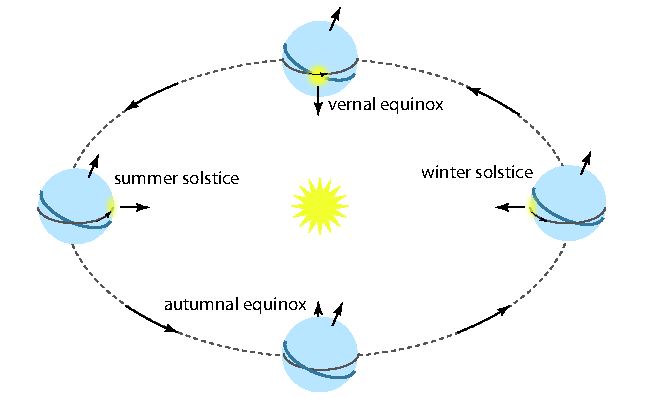
\includegraphics[width=\linewidth]{ecliptic}
\caption[The ecliptic]{As Earth orbits the Sun, the Sun's declination traces out a path along the celestial sphere known as the \emph{ecliptic}.  Over the course of a year, the Sun appears to move eastward, relative to distant stars, along the ecliptic.}
\label{f.ecliptic}
\end{figure}

The Sun reaches its minimum declination, \dec{-23}{16}{}, when it appears to lie in the direction of Sagittarius at the \emph{winter solstice}.  One quarter orbit later, the Sun crosses the celestial equator; at this point the Sun is in the direction of Pisces at the \emph{vernal equinox}. Another quarter orbit brings the Sun in the direction of Gemini with declination \dec{23}{16}{}; this is the \emph{summer solstice}. A further quarter orbit, and the Sun crosses the celestial equator in the direction of Virgo at the \emph{autumnal equinox}.

The ecliptic thus intersects the celestial equator at two points (Fig.~\ref{f.ecliptic}), the \emph{vernal and autumnal equinoxes}. We usually associate the equinoxes with a specific time of year, but they actually define unique directions on the sky. We can therefore define our second angular coordinate, \emph{right ascension}, as the angle between an objects' meridian and the vernal equinox, measured eastwards along the celestial equator.

\begin{marginfigure}
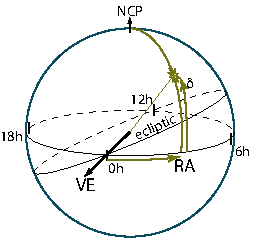
\includegraphics[width=\linewidth]{right-ascension}
\caption[Right ascension and declination]{The right ascension (\RA) and declination ($\delta$) of a celestial object.}
\label{f.right-ascension}
\end{marginfigure}

Rather than specify the right ascension by degrees, astronomers instead quote it in terms of hours (and minutes and seconds).  The vernal equinox is therefore at $\RA = \hrangle{00}{00}{00}$ and the autumnal equinox is at $\RA = \hrangle{12}{00}{00}$.

\begin{exercisebox}[Current right ascension of the Sun and Betelgeuse]
Estimate the Sun's current right ascension.  Given that Betelgeuse is currently visible in the night sky, what is a a plausible value for its right ascension?
\label{ex.RA-sun}
\end{exercisebox}

\section{Precession}
As we noted above, at the summer solstice, the Sun is in the direction of Gemini. On the solstice, the Sun will appear to be directly overhead at a latitude of \dec{23}{16}{}N, which is known as the \emph{Tropic of Cancer}.  Why isn't it called the Tropic of Gemini?

The answer is that the Earth's rotation axis is not fixed; it precesses. The north and south celestial poles trace a circle on the sky relative to distant stars over a $\val{26\,000}{\yr}$ period. The causes the direction of the equinoxes to move westward along the ecliptic on that timescale.  There are 13 constellations, the \emph{zodiac}, around the ecliptic; in the last two millennia the direction of the summer solstice has shifted one constellation over, from Cancer to Gemini.  Likewise, the winter solstice used to be in the direction of Capricorn; now it is in the direction of Sagittarius.

As a practical matter, this means that the coordinates of right ascension and declination, which are based on the direction of the Earth's rotation axis, slowly change.  To account for this, when giving the coordinates for an object astronomers specify an \emph{epoch}---a reference time to which the right ascension and declination refer. The current epoch is J2000, which refers to roughly noon UTC on 1 January 2000.

\begin{exercisebox}[Coordinate systems]
Brainstorm some possible coordinate systems, and describe their advantages and disadvantages in comparison to right ascension and declination.
\end{exercisebox}

\section{Keeping time}

Our \emph{local noon} is when the Sun crosses our meridian\sidenote{The local noon is usually \emph{not} at 12:00pm: our time zones are only to the nearest hour, and there is an adjustment for daylight savings time.}. The time between two successive noons is one \emph{solar day}, which we divide into 24 hours. This is slightly longer than the time for the earth to complete one rotation, however: because of the Earth's motion about the Sun, the position of the Sun shifts by about one degree over the course of a day, and the Earth must rotate that amount in addition to one full rotation before the next noon (Fig.~\ref{f.solar-day}).

\begin{marginfigure}
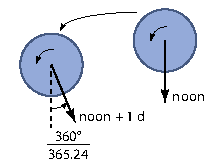
\includegraphics[width=\linewidth]{solar-day}
\caption[The movement of the Earth from noon to noon]{The movement of the Earth from noon to noon.  The arrows indicate the direction towards the Sun.}
\label{f.solar-day}
\end{marginfigure}

There are $365.24$ solar days between successive solar crossings of the vernal equinox, which defines a \emph{tropical year}.  Over the course of this year, the extra rotation on each solar day adds up to one complete rotation of the Earth.  The Earth rotates $366.24$ times in one tropical year, and therefore the rotation period of the Earth is
\[ \frac{365.24}{366.24}\times \val{24}{\hour} =  \hrangle{23}{56}{04}.  \]
In fact, the tropical year is slightly shorter, by about $\val{20}{\minute} = \val{1}{\yr}/26\,000$ because of the precession of the Earth's axis.

Our time---hours and minutes---is tied to the position of the Sun, which is convenient for daily activity but not so convenient if we want to know when a particular star is observable.  Instead of marking when the Sun crosses our meridian, we define our local \emph{sidereal time} relative to our meridian crossing the vernal equinox.  Because we also define right ascension relative to the vernal equinox, objects with a right ascension near that of the sidereal time will be high in the sky.

To compute our local sidereal time, first determine the right ascension of the Sun (Exercise \ref{ex.RA-sun}); this will then fix the offset between the local sidereal time and the local noon in UTC.  We can then compute our offset for local noon based on our longitude.

\begin{exercisebox}[Current sidereal time]
Local noon at $0^{\circ}$ longitude corresponds to 12:00 UTC. Given that our longitude is $\dec{84}{28}{33}\,\mathrm{W}$, what is our local noontime in UTC.  What local time would this correspond to today? From this and your estimate of the Sun's current hour angle, what is the current sidereal time?
\end{exercisebox}

\section{Parallax}

The motion of the Earth around the Sun \emph{does} cause a small shift in the apparent angular position of a star, a phenomena known as \emph{parallax}.  This effect is exploited to determine the distance to nearby stars.  

\begin{figure*}[htb]
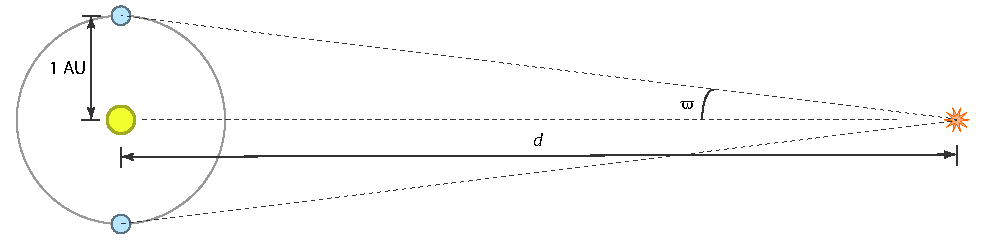
\includegraphics[width=\linewidth]{parallax}
\caption[The parallax angle of a star]{The parallax angle $\varpi$ of a star induced by Earth's motion around the Sun.}
\label{f.parallax}
\end{figure*}

The angular shift, $\varpi$, is related (see Fig.~\ref{f.parallax}) to the radius of the Earth's orbit, \val{1}{\AU}, and the distance to the star $d$ via
\[
\frac{\val{1}{\AU}}{d} = \tan\varpi \approx \varpi.
\]
When $\varpi$ is expressed in arcseconds, this gives
\begin{equation}\label{e.parallax}
d = \frac{\val{206\,265}{\AU}}{\varpi/1''} = \val{1}{\parsec}\left(\frac{1''}{\varpi}\right) ,
\end{equation}
which defines the \emph{parsec}.  In CGS units $\val{1}{\parsec} = \val{\sci{3.086}{18}}{\cm}$, which is a bit over 3 light-years.

\section{Angular distances between nearby objects}

To compute the angular distance between two points on the sky, we draw two vectors $\bvec{a}$, $\bvec{b}$ to these points and use
\[ \cos\theta = \frac{\bvec{a}\vdot\bvec{b}}{|\bvec{a}||\bvec{b}|}. \]
Since both $\bvec{a}$ and $\bvec{b}$ lie on the unit sphere, $|\bvec{a}| = |\bvec{b}| = 1$; the $(x,y,z)$ components of these vectors are
\[
\left(\cos\delta_{1}\cos\eta_{1}, \cos\delta_{1}\sin\eta_{1}, \sin\delta_{1}\right)
\]
and
\[
\left(\cos\delta_{2}\cos\eta_{2}, \cos\delta_{2}\sin\eta_{2}, \sin\delta_{2}\right),
\]
respectively. 
Taking the dot product,
\begin{eqnarray}
\cos\theta &=& \cos\delta_{1}\cos\delta_{2}\left(\cos\eta_{1}\cos\eta_{2} + 
	\sin\eta_{1}\sin\eta_{2}\right) + \sin\delta_{1}\sin\delta_{2}\nonumber\\
	 &=& \cos\delta_{1}\cos\delta_{2}\cos\left(\eta_{1}-\eta_{2}\right) + 
	 	\sin\delta_{1}\sin\delta_{2}.
\label{e.angular-distance}
\end{eqnarray}

\begin{marginfigure}[-14\baselineskip]
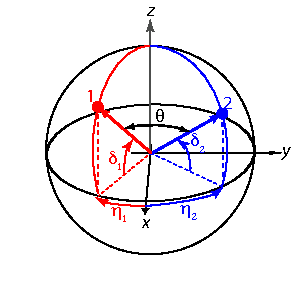
\includegraphics[width=\linewidth]{angular-distance}
\caption[Angular distance between two points on a sphere]{Two locations on the sphere separated by a distance $\theta$.}
\label{f.angular-distance}
\end{marginfigure}

We are usually interested in the angular distance between two nearby sources, with RAs $\eta_{1} \approx \eta_{2}$ and declinations\sidenote{Notice our coordinates differ from the usual spherical polar coordinates: $\delta$ is measured from the $x$-$y$ plane, not from the $z$-axis.} $\delta_{1}\approx\delta_{2}$.  We can use the expansion rule,
\[ \cos x \approx 1 - \frac{x^{2}}{2},\qquad x \ll 1 \, \]
on $\theta$ and $\eta_{1}-\eta_{2}$ in equation~(\ref{e.angular-distance}):
\begin{eqnarray*}
	1-\frac{\theta^{2}}{2} &\approx& \cos\delta_{1}\cos\delta_{2} \left[1-\frac{(\eta_{1}-\eta_{2})^{2}}{2}\right] + \sin\delta_{1}\sin\delta_{2}\\
		&=& \cos(\delta_{1}-\delta_{2}) - \cos\delta_{1}\cos\delta_{2}\frac{(\eta_{1}-\eta_{2})^{2}}{2}.
\end{eqnarray*}
We can now expand $\cos(\delta_{1}-\delta_{2})$, cancel common factors and multiply by 2,
\[ \theta^{2} \approx (\delta_{1}-\delta_{2})^{2} + \cos\delta_{1}\cos\delta_{2}(\eta_{1} - \eta_{2})^{2}. \]
Finally, we notice that to lowest order, $\cos\delta_{1}\cos\delta_{2}\approx \cos^{2}\delta$, where $\delta = (\delta_{1}+\delta_{2})/2$ is the average of the two declinations.  This gives us a formula for the angular distance $\theta$ between two nearby points,
\marginnote{%
We make heavy use of the sine and cosine addition formula: $\cos(x+y) = \cos x\cos y - \sin x\sin y$, and $\sin(-y) = -\sin y$, $\cos(-x) = \cos(x)$.}
\begin{equation}
\theta \approx \sqrt{\cos^{2}\delta\left(\eta_{1}-\eta_{2}\right)^{2} + \left(\delta_{1}-\delta_{2}\right)^{2}}.
\end{equation}
This looks like the pythagorean formula; the factor of $\cos\delta$ accounts for the lines of constant RA converging as they approach the poles.

\begin{marginfigure}[4\baselineskip]
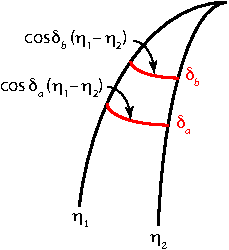
\includegraphics[width=\linewidth]{angular-distance2}
\caption[Angular distance between lines of constant right ascension]{The distance between two RAs $\eta_{1}$ and $\eta_{2}$, measured along a circle of radius $\cos\delta$.}
\label{f.angular-pythagorean}
\end{marginfigure}

\begin{exercisebox}[Angular size of the Pleiades]
Atlas A and Electra are two bright stars that lie on the east and west sides of the Pleiades star cluster.  Atlas has right ascension $\RA = \hrangle{03}{49}{09.7}$ and declination $\delta = \dec{24}{03}{12}$; Electra has $\RA = \hrangle{03}{44}{52.5}$ and $\delta = \dec{24}{06}{48}$.  Find the angular distance between these stars.  If the distance to the Pleiades is $\val{136}{\parsec}$, what is the projected distance between these stars?
\end{exercisebox}

\section{Looking up}
Finally a note about directions when looking up at the sky.  We've drawn our coordinates from the perspective of someone outside the celestial sphere; our perspective, however, is from the center.  When we look up at the sky, if we face south, so that the direction northwards is at the top of our field of view, then the easterly direction is to our \emph{left}. Objects of larger right ascension are therefore to our left as well.
